\chapter{Moses}

Moses je statistický překladový systém založený na překladu frází (anglicky PBMT - phrase-based machine translation). 

\section{Princip frázového překladu}

\begin{figure}[ht]
\begin{center}
\includegraphics[scale=0.5,bb=36 36 416 186]{pictures/phrase-based.eps}
\end{center}
\caption{Architektura frázových překladových systémů.}
\label{phrase-based-models}
\end{figure}

Součastné nejvyspělejší generické (tedy více či méně nezávislé na jazykovém páru) překladové systémy jsou založeny na překladu frází. Jejich architektura je znázorněna na Obrázku \ref{phrase-based-models}.

\section{Jazykový a překladový model}
Tyto systémy používají k překladu vstupu na výstup překladový a jazykový model. Překladový model zachycuje četnost překladů frází délky n. Tyto fráze jsou také označovany jako n-gramy. Překladový model lze získat z paralelních korpusů, tedy přeložených textů mezi zdrojovým a cílovým jazykem. Jazykový model zachycuje četnost výskytu frází v cílovém jazyce. Pro jeho získání tedy stačí texty v cílovém jazyce. Díky překladovému a jazykovému modelu lze získat různé překlady frází ve vstupním textu. Pro vygenerování výstupu potřebuje překladový systém nalézt posloupnost frází v cílovém jazyce, které pokrývají všechny části vstupu a mají největší pravděpodobnost výskytu.

\section{Hledání nejlepších hypotéz}
Při generování překladu používá Moses strukturu, která se anglicky nazývá "lattice", neboli graf slov.

Variant překladu může být obecně exponenciální množství. Pro rychlé hledání v těchto variantách implementuje Moses tzv. beam search algoritmus. Postup algoritmu při hledání zobrazuje Obrázek 2.2. Jedná se vlastně o orientovaný graf. Vrcholy grafu znázorňují částečné hypotézy. Každá taková částečná hypotéza pokrývá nějaká slova ze vstupu a má skóre, které určuje kvalitu hypotézy. Na začátku je překladu je prázdná hypotéza, která nepokrývá žádnou část vstupu. Na konci máme hypotézy které pokrývají celý vstup. Během překladu překladový systém postupně rozšiřuje exitující hypotézy o další fráze. Hypotéza s nejvyšším skóre je nabídnuta jako překlad na výstup. Pomocí tabulky překladovýchmožností dokáže Moses poskytnou i další hypotézy seřazené podle pravděpodobnosti.

\section{Rozšíření Mosese}
Pro poskytnutí nápovědy během překladu bylo nutné rozšířit možnosti Mosese tak, aby dokázal generovat hypotézy z neprázdné počáteční hypotézy. Překladatel je uprostřed překladu věty, má přeložená určitá slova a potřebuje radu, jak nejlépe pokračovat dál. Pomocí implementovaného rozšíření se nyní může zeptat Mosese, který může začít generovat překlad navazující na již přeloženou část. K tomu potřebuje vektor označující části vstupní věty, které byly již přeloženy. Kvůli jazykovému modelu, který kontroluje, aby navazující část byla v cílovém jazyce co nejvíce smysluplná, potřebuje Moses znát část přeloženého textu, na kterou se může pokusit navázat. Pomocí tohoto rozšíření může Moses začít rozvíjet hypotézy, které se v prvotním překladu z prázdné hypotézy nemusely vůbec objevit. Toto by mělo přispět k flexibilitě nápovědy. Správný překlad totiž leckdy může být specifický a použitá slova nemusí být v překladovém modelu vůbec použita.









